\documentclass{article}
\usepackage[margin=1in]{geometry}
\usepackage{graphicx}
\usepackage{tikz}
\usetikzlibrary{arrows}
\usepackage{multicol}

\newcommand{\vect}[1]{\langle #1 \rangle}
\begin{document}
\noindent{\bf CSCI 480, Fall 2015, Math Homework \# 3}
\\Due date:  Friday, December 11, midnight
\bigskip

\noindent Name\hrulefill Number \hrulefill

Typeset this homework using \LaTeX.  Pictures can be hand drawn,
scanned, and included as images (see the jpg below).

\begin{enumerate}

\item Express the homogeneous 3D transformation defined by the matrix
  \[
\left[  \begin{array}{cccc}
    0 & -1 & 0 & 2 \\
    1 & 0 & 0 & 3 \\
    0 & 0 & 1 & 4 \\
    0 & 0 & 0 & 1\\\end{array}\right]
\]
As a sequence of transformations in the following ways.
Express your answer in English as well as two simpler transformation
matrices.
\begin{enumerate}
\item  A rotation followed by a translation.
\item A translation followed by a rotation.
  \end{enumerate}

\item
  \begin{multicols}{2}
    The pyramid shown is represented by the following vertices:
  \begin{eqnarray*}
    0 &:& (0,1,0,0)\\
    1 &:& (1,0,0,0)\\
    2 &:& (0,0,1,0)\\
    3 &:& (-1,0,0,0)\\
    4 &:& (0,0,-1,0)
    \end{eqnarray*}
\columnbreak
  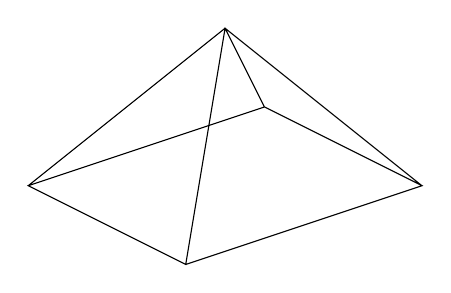
\begin{tikzpicture}
    \draw (2,1) -- (5,2) -- (3,3) -- (0,2) -- (2,1)
          -- (2.5,4) -- (5,2) (3,3) -- (2.5,4) -- (0,2);
  \end{tikzpicture}
  \end{multicols}
    We assume a standard OpenGL frame.
  \begin{enumerate}
  \item
    Give an elements list that describes the top four triangles, being
  careful to make each of them face outward.
\item Give an elements list that describes the bottom square as two
  triangles, both of which include the point numbered 1.  Again, make
  sure they face outward (in this case, down).
  
  \end{enumerate}
  \begin{multicols}{2}
\item
    The Eiffel tower is 300 meters high.  Let's assume that the girl
    in the picture is 1 meter tall.  If the girl is 10 meters from the
    camera, approximately how far away is the Eiffel tower?
    Draw pictures to explain your answer.

    If we're going to try to recreate this in OpenGL, and the {\em
      near} distance is set to $x$, what would be good values for
    the {\em top} and {\em bottom} distances?
    Draw pictures to explain your answer.

    \vfill

\columnbreak
  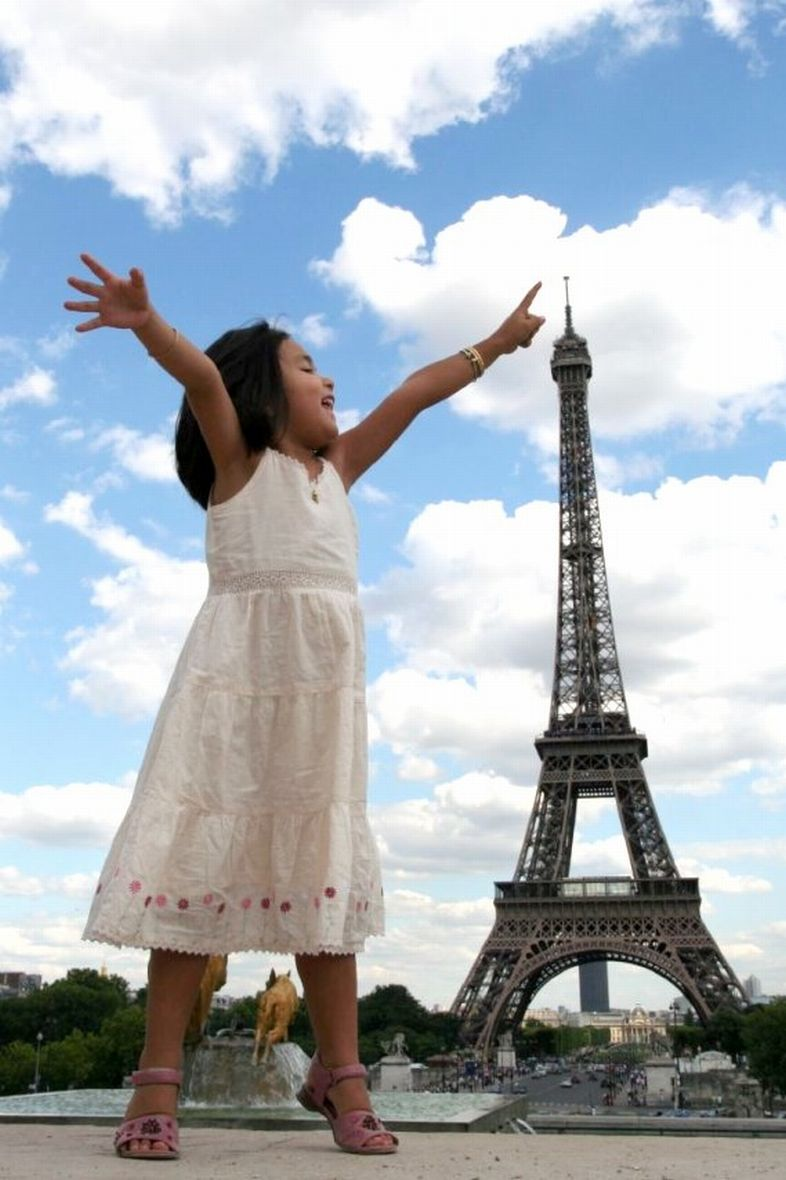
\includegraphics[scale=0.125]{27.jpg}
  \end{multicols}
  
\item A camera is placed at $(5,0,0)$ looking at the origin.  It's
  {\em up} vector is the $y$ axis.  What is
  the camera's {\em view} matrix?
\end{enumerate}
\end{document}
